\documentclass[11pt, a4paper]{article}

\usepackage{amsmath}
\usepackage{hyperref}
\usepackage{graphicx}
\usepackage{listings}
\usepackage{color}

\author{
  \textbf{KOTWAL ALANKAR SHASHIKANT}\\
  \texttt{12D070010}
  \and
  \textbf{ANAND KALVIT}\\
  \texttt{12D070032}
}
\title{Visual Odometry from Stereo Using Point-Set Matching}

\begin{document}
\maketitle
\newpage

\section{Introduction}
Odometry refers to the use of data from motion sensors to estimate change in position over time. One of the most reliable ways of estimation of 3-D structure using cameras is to use a calibrated stereo pair. Given the sequence of 3-D structures generated by the stereo camera, we can estimate the motion of the camera with respect to its environment as well as generate a 3-D map of the environment. This is usually referred to as visual SLAM (simultaneous localization and mapping), which has wide applications in robotics and remote sensing. \\

\noindent We plan to implement a 6 DoF pose estimation algorithm using a calibrated stereo pair and generate a 3-D map of the environment simultaneously. We assume that scene illumination doesn't change much and most of the field of view of the camera is occupied by static parts of the environment. \\

\noindent In a nutshell, our job is to figure out what the translation and rotation of the camera is between two scenes as shown below. \\ \\ \\
\centerline{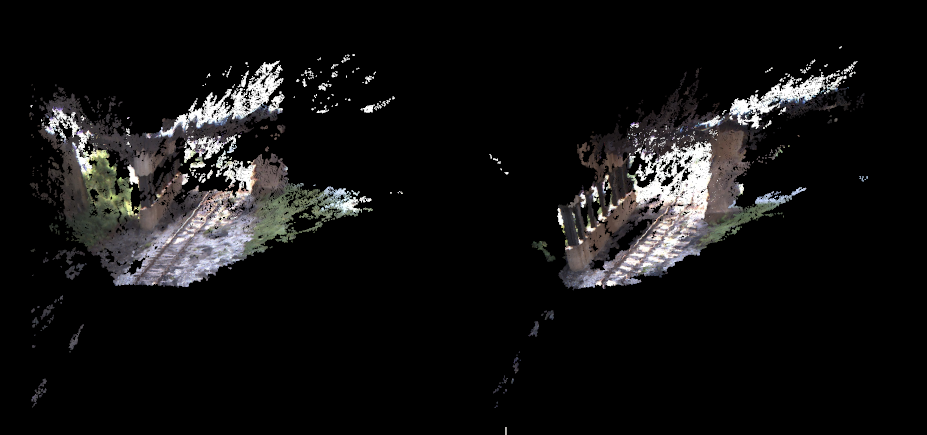
\includegraphics[scale=0.50]{pointclouds}}
\newpage

\section{Method}
We closely follow the method outlined in \cite{main}. The method involves modelling both the reference and the moving pointclouds as Mixture Models. We choose spherical Gaussian Mixtures and equal weights per-point for simplicity and easy updates. Our model for the pointclouds, thus, is given by $$\mathcal{S}(\textbf{x}) = \sum_{i=1}^N \mathcal{G}(\textbf{x}; \textbf{s}_i, \Sigma), \mathcal{M}(\textbf{x}) = \sum_{i=1}^M \mathcal{G}(\textbf{x}; \textbf{m}_i, \Sigma)$$ where $N = |\mathcal{S}|, M = |\mathcal{M}|, \Sigma = diag(\sigma^2)$. We then maximise the kernel correlation between a translated and rotated version of the moving pointcloud and the reference pointcloud, with respect to the rotation and the translation, yielding the optimization problem $$\textbf{R}, \textbf{t} = arg\max_{\textbf{R}, \textbf{t}} \sum_{i=1}^M \sum_{j=1}^N e^{-\frac{|| \textbf{Rx}_i + \textbf{t} - \textbf{y}_j ||^2}{2 \sigma^2}}$$ such that $\textbf{R}^T \textbf{R} = I$. This is a convex program and the optimization is carried out using gradient ascent on the components of $\textbf{t}$ and a parametrization of the rotation matrix $\textbf{R}$, as described in the implementation section below.

\section{Implementation}
We chose to code the method in C++ using PCL to handle pointcloud representation and i/o, and Eigen to handle the matrix algebra. With this, we chose to represent rotations using unit quaternions to make gradient-descent optimization convenient and avoid the orthogonality constraint on \textbf{R}.
\linebreak \linebreak
\noindent Gradient ascent requires us to calculate the gradient of the objective function with respect to the optimizing variables. With the help of \cite{mainPre} (see appendix 2), we get, with $F(\mathcal{S}, \mathcal{M}, \textbf{R}, \textbf{t})$ being the objective function defined above, $$\frac{\partial F}{\partial \textbf{t}} = \textbf{G}^T\textbf{1}_m$$ $$\frac{\partial F}{\partial r_i} = \textbf{1}_d^T \left(\textbf{G}^T\textbf{M}_0 \otimes \frac{\partial \textbf{R}}{\partial r_i}\right)\textbf{1}_d$$ where $(r_0, r_1, r_2, r_3)$ is the unit-quaternion representation of the rotation matrix.
\linebreak \linebreak
\noindent
The derivatives of $\textbf{R}$ with respect to $r_i$ are calculated, from \cite{quatParam} as
$$\frac{\partial \textbf{R}}{\partial r_0} = 2\begin{pmatrix}
  r_0 & -r_3 & r_2 \\
  r_3 & r_0 & -r_1 \\
  -r_2 & r_1 & r_0
 \end{pmatrix}$$
$$\frac{\partial \textbf{R}}{\partial r_1} = 2\begin{pmatrix}
  r_1 & r_2 & r_3 \\
  r_2 & -r_1 & -r_0 \\
  r_3 & r_0 & -r_1
 \end{pmatrix}$$
$$\frac{\partial \textbf{R}}{\partial r_2} = 2\begin{pmatrix}
  -r_2 & r_1 & r_0 \\
  r_1 & r_2 & r_3 \\
  -r_0 & r_3 & -r_2
 \end{pmatrix}$$
$$\frac{\partial \textbf{R}}{\partial r_3} = 2\begin{pmatrix}
  -r_3 & -r_0 & r_1 \\
  r_0 & -r_3 & r_2 \\
  r_1 & r_2 & r_3
 \end{pmatrix}$$


\noindent Apart from this, we used adaptive step-size to prevent overshoot and slow convergence.

\section{Results}
\subsection{Generating pointclouds from stereo images}
See pointclouds in \textit{pointclouds/*}. The original images had a resolution of 640 $\times$ 512 pixels, so the original pointclouds had of the order of $10^5$ points. This is too much for us to process, so we down-sample the pointclouds by a factor of $\sim$100 to reduce the number to a manageable quantity.

\subsection{Estimating identity transformations}
The first checkpoint is checking if the code estimates the transformation between identical pointclouds correctly. We save the output rotation matrix in \textit{data/tfxxR.transform} and the output translation in \textit{data/tfxxt.transform} where x is the pointcloud number. For example, the estimated identity transformation for the pointcloud \textit{pair00.pcd} is $$\hat{\textbf{R}} = \begin{pmatrix}
1 & -7.72142 \times 10^{-10} & 7.72142 \times 10^{-10} \\
7.72142 \times 10^{-10} & 1 & 1.26552 \times 10^{-8} \\
-7.72142 \times 10^{-10} & -1.26552 \times 10^{-8} & 1
 \end{pmatrix}$$ and $$\hat{\textbf{t}} = \begin{pmatrix}
8.77619 \times 10^{-10} \\
1.20335 \times 10^{-11} \\
4.22396 \times 10^{-11}
 \end{pmatrix}$$

\noindent As is clear, these are very close to the identity transformation, confirming that the method estimates identity transformations properly. We sometimes have convergence problems (especially for large rotation angles). The plot of the objective function (starting from some initialization) is shown below: \\ \\
\centerline{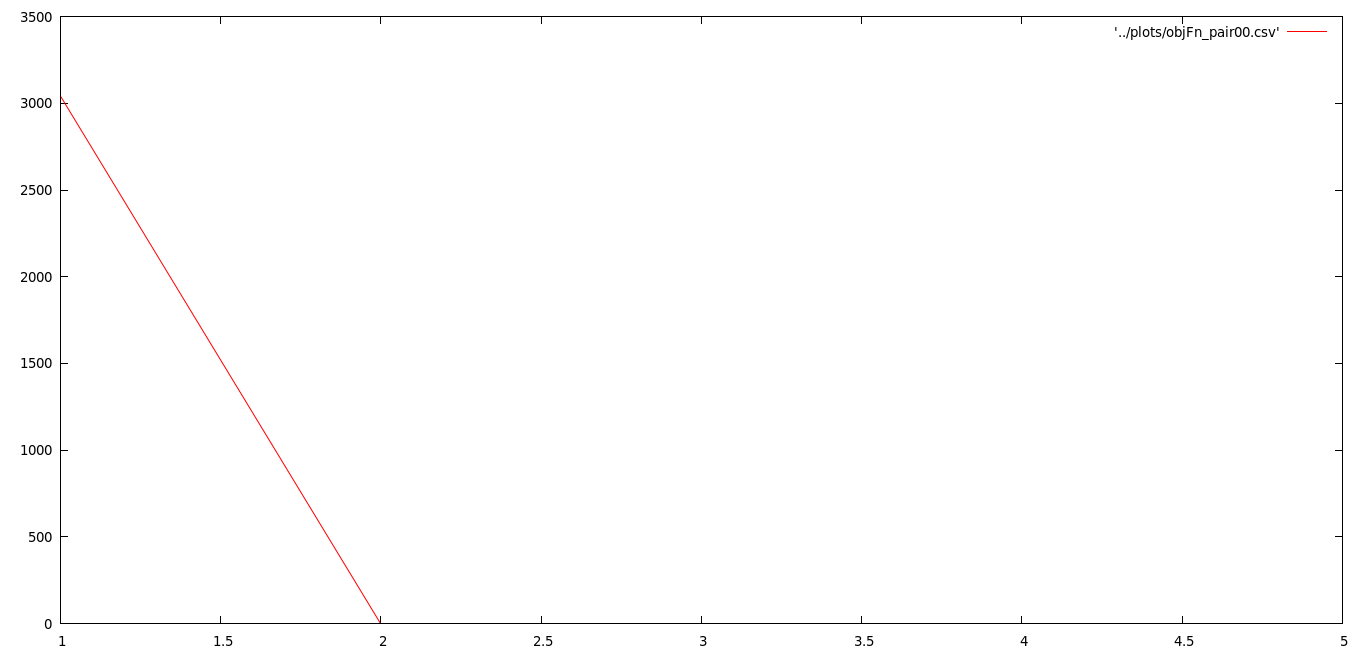
\includegraphics[scale=0.35]{objFn_pair00}}

\subsection{Estimating synthetic transformations} 
As the next step, we `synthesize' transformed pointclouds (by translating and rotating one of the pointclouds by known quantities). For example, the transformation matrix
$$T = \begin{pmatrix}
 1 & 0 & 0 & 250 \\
 0 & 1 & 0 & 0 \\
 0 & 0 & 1 & 0 \\
 0 & 0 & 0 & 1
\end{pmatrix}$$
on the pointcloud \textit{pair00.pcd} yields the two pointclouds (one white and one green) as shown: \\ \\
\centerline{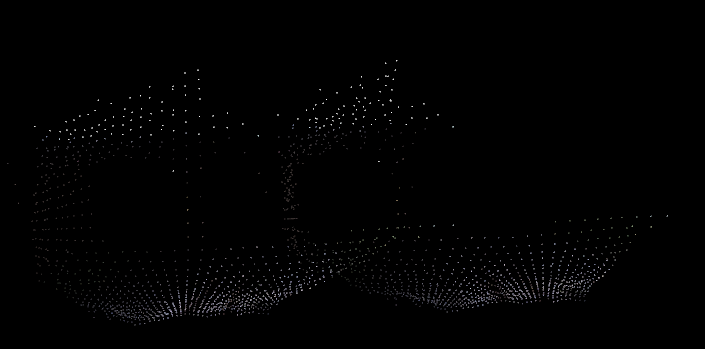
\includegraphics[scale=0.5]{dispSynthPair}} \\ \\
We then run the matching algorithm on these pointclouds and compare the output to the (known) transformation matrix. For this particular example, the estimated transformation after twenty iterations (the estimate was initialised at -245) is
$$T = \begin{pmatrix}
 1 & 0 & 0 & 249.903 \\
 0 & 1 & 0 & 0 \\
 0 & 0 & 1 & 0 \\
 0 & 0 & 0 & 1
\end{pmatrix}$$
which is close enough to the original value. A plot of the objective function with iteration number is shown below: \\ \\
\centerline{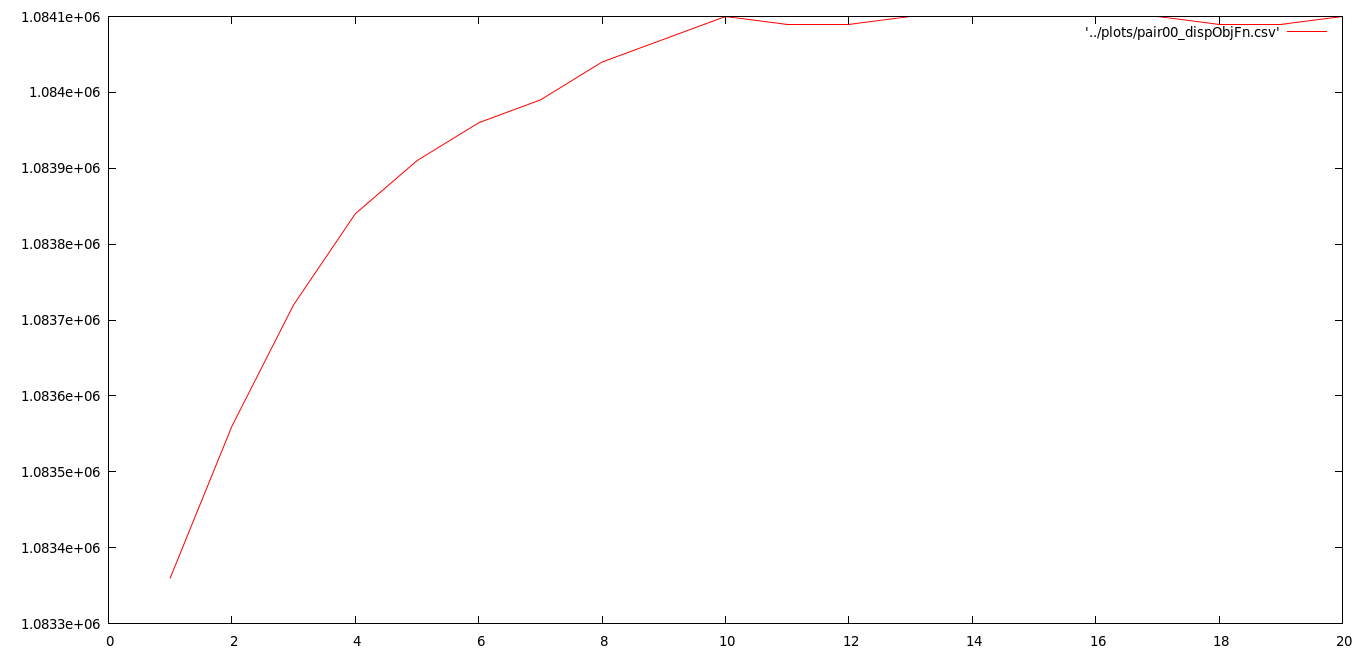
\includegraphics[scale=0.35]{pair00_dispObjFn}} \\ \\
The value of the x-component of the displacement is shown below: \\ \\
\centerline{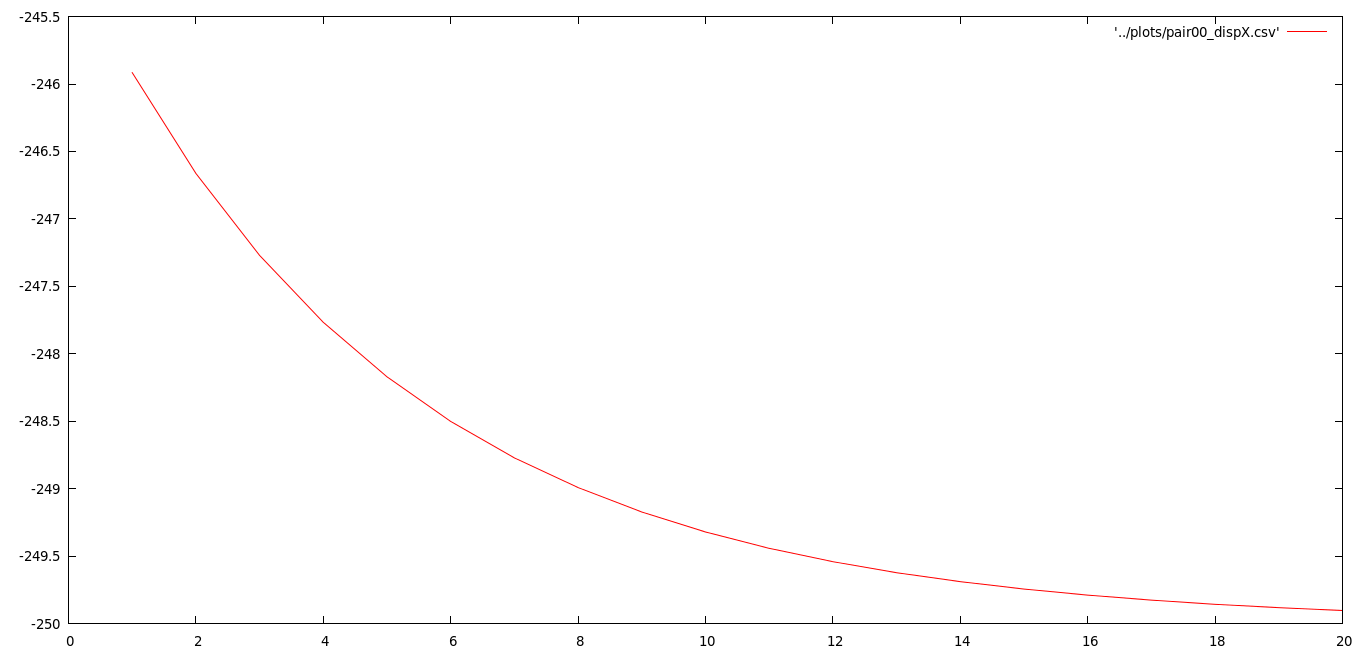
\includegraphics[scale=0.35]{pair00_dispX}} \\ \\

\noindent A similar experiment with a pointcloud rotated at $30^0$, shown below, yields the following objective-function graph: \\ \\
\centerline{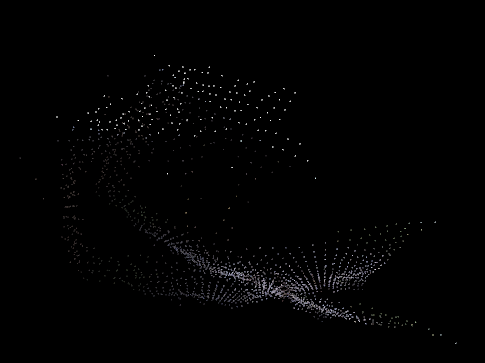
\includegraphics[scale=0.75]{rotSynthPair}}  \\ \\
\centerline{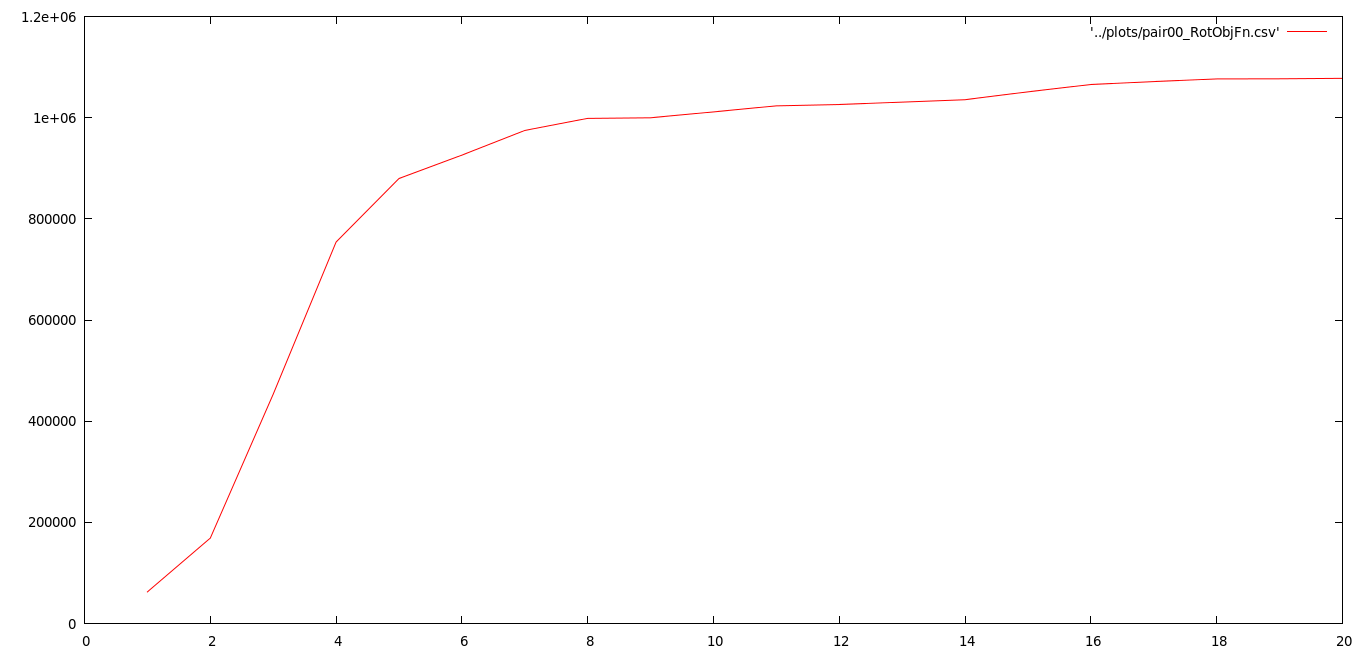
\includegraphics[scale=0.35]{pair00_rotObjFn}} \\ \\

\subsection{Estimating transformations between different pointclouds}
Now we try to estimate the transformation between different pointclouds. Here we have significant convergence problems if the transformation is not initialised sufficiently close to the actual transformation. We think this is because the pointclouds used have relatively little overlap, and this is not sufficient to make the algorithm converge to the actual transformation. We weren't able to get convergence with the data we had. We do not include the results since we do not think this part is complete.

\section{Other Methods}
We also tried an implementation of Coherent Point Drift, see \cite{cpd} and \cite{wiki}, which we did not get time to debug and test. This is in a non-working state right now.

\section{Concluding Remarks}
We showed the algorithm working for the identity transformation and transformations that don't differ much from identity. However, estimation of small transformations is useful enough since two pointclouds which are captured in succession are related by transformations that are not very different from each other.
\newline \linebreak
\noindent There are a few problems with the method. In order to obtain results with almost any non-identity transformation, we need to tune the variance, the step-size, and the step-size adjustment parameters for the adaptive part to get good results. Almost always, we need to initialize the estimate at a point that is close enough to the actual transformation to avoid getting lost in the parameter space.

\begin{thebibliography}{9}

\bibitem{main}
  Bing Jian and Vemuri, B.C.,
  \emph{Robust Point Set Registration Using Gaussian Mixture Models}.
  IEEE Transactions on Pattern Analysis and Machine Intelligence,
  2010.
  
\bibitem{mainPre}
  Pre-print of the above paper \href{http://code.google.com/p/gmmreg/downloads/detail?name=gmmreg_PAMI_preprint.pdf}{here}.
  
\bibitem{quatParam}
  George Terzakis, Phil Culverhouse \textit{et al},
  \emph{A Recipe on the Parametrization of Rotation Matrices for Non-Linear Optimization using Quaternions}.
  Technical Report of the School of Marine Science and Engineering, Plymouth University,
  2012.
  
\bibitem{cppStuff}
  Documentation for the OpenCV, Point Cloud and Eigen libraries in C++ \href{http://docs.opencv.org/}{here},\href{http://pointclouds.org/documentation/}{here} and \href{http://eigen.tuxfamily.org/dox/}{here} respectively

\bibitem{cpd}
  Andriy Myronenko and Xubo Song,
  \emph{Point Set Registration: Coherent Point Drift}.
  IEEE Transactions on Pattern Analysis and Machine Intelligence,
  2010.

\bibitem{wiki}
  The Wikipedia article on Point Set Registration \href{http://en.wikipedia.org/wiki/Point_set_registration}{here}.

\end{thebibliography}

\section*{Appendix 1}
Here we derive the expression for the kernel correlation between two Gaussian mixtures. Following \cite{main} we want to evaluate the integral $$\int_{\mathcal{R}^3} f_{\textbf{R, t}} g d\textbf{x}$$ with $f$ and $g$ being Gaussian mixtures with means $\textbf{s}_i$ and $\textbf{m}_i$ respectively. We assume uncorrelated Gaussians, so covariance everywhere is $\sigma^2 \textbf{I}$. Thus, the correlation becomes, \textit{modulo} constants, $$\sum_{i=1}^{N} \sum_{j=1}^{M} \int_{\mathcal{R}^3} e^{\frac{|| \textbf{x} - \textbf{Rs}_i - \textbf{t} ||^2 + || \textbf{x} - \textbf{m}_j ||^2}{2 \sigma^2}}$$ The numerator of the exponential can be written as $$\left( \textbf{x} - \textbf{Rs}_i - \textbf{t} \right)^T \left( \textbf{x} - \textbf{Rs}_i - \textbf{t} \right) + \left( \textbf{x} - \textbf{m}_j \right)^T \left( \textbf{x} - \textbf{m}_j \right)$$ With $\textbf{Rs}_i + \textbf{t} \textbf{n}_i$,
$$\left( \textbf{x} - \textbf{m} \right)^T \left( \textbf{x} - \textbf{m} \right) + \left( \textbf{x} - \textbf{n} \right)^T \left( \textbf{x} - \textbf{n} \right)$$ which is the same as $$2\left( \textbf{x} - (\textbf{m}+\textbf{n}) \right)^T \left( \textbf{x} - (\textbf{m}+\textbf{n}) \right)$$ which makes the correlation the sum of Gaussian functions with mean $\textbf{RS}_i + \textbf{t} - \textbf{m}_j$ evaluated at zero. So $$\int_{\mathcal{R}^3} f_{\textbf{R, t}} g d\textbf{x} = \mathcal{K} \sum_{i=1}^{N} \sum_{j=1}^{M} e^{-\frac{|| \textbf{Rs}_i + \textbf{t} - \textbf{m}_j ||^2}{2 \sigma^2}}$$ where $\mathcal{K}$ is a positive constant independent of \textbf{R} or \textbf{t}.

\section*{Appendix 2}
Here we derive the expressions for the gradient descent technique used in the registration method.
\newline \linebreak
\noindent The optimization problem under consideration is $$\textbf{R}, \textbf{t} = arg\min_{\textbf{R}, \textbf{t}} \sum_{i=1}^M \sum_{j=1}^N e^{-\frac{|| \textbf{Rx}_i + \textbf{t} - \textbf{y}_j ||^2}{2 \sigma^2}}$$ such that $\textbf{R}^T \textbf{R} = I$. To calculate the derivative of this quantity with respect to the optimization variables \textbf{R} and \textbf{t}, we use the chain rule:
$$\frac{\partial F}{\partial q} = \frac{\partial F}{\partial M} \frac{\partial M}{\partial q}$$ where $M$ is the transformed data-set and $q$ is the optimization variable under consideration. Now with $\textbf{m}_t$ being the transformed version of $\textbf{x}_t$, $$\frac{\partial F}{\partial \textbf{m}_t} = \sum_{j=1}^N \frac{\partial}{\partial \textbf{m}_t} e^{-\frac{|| \textbf{m}_t - \textbf{y}_j ||^2}{2 \sigma^2}}$$ thus yielding $$\frac{\partial F}{\partial \textbf{m}_t} = -\sum_{j=1}^N \frac{e^{-\frac{|| \textbf{m}_t - \textbf{y}_j ||^2}{2 \sigma^2}}}{\sigma^2} \left( \textbf{m}_t-\textbf{y}_j \right)^T$$ The matrix consisting of M of these row vectors is what we called $\textbf{G}^T$.
\newline \linebreak
\noindent Clearly, $$\frac{\partial \textbf{m}_i}{\partial t_x} = \frac{\partial \left(\textbf{Rs}_i + \textbf{t}\right)}{\partial t_x}$$ which is just 1. So, the derivative of $F$ with respect to $\textbf{t}$ is just $\textbf{G}^T \textbf{1}_M$ where $\textbf{1}_M$ is the column vector of all ones, corresponding to adding up the derivatives with respect to all $\textbf{m}_t$s.
\newline \linebreak
\noindent Figuring out the derivative with respect to rotation is a bit more difficult since we have a constraint on the rotation matrix. To avoid having to explicitly enforce this constraint we use a quaternion parametrization of the rotation matrix. Following the excellent treatment in \cite{quatParam}, we have the rotation matrix induced by the quaternion $\textbf{q} = (q_0, q_1, q_2, q_3)$ is
$$\textbf{R} = \begin{pmatrix}
q_0^2 + q_1^2 + q_2^2 + q_3^2 & 2(q_1 q_2-q_0 q_3) & 2(q_1 q_3 + q_0 q_2) \\
2(q_1 q_2 + q_0 q_3) & q_0^2 - q_1^2 + q_2^2 - q_3^2 & 2(q_2 q_3 - q_0 q_1) \\
2(q_1 q_3 - q_0 q_2) & 2(q_2 q_3 + q_0 q_1) & q_0^2 - q_1^2 - q_2^2 + q_3^2
\end{pmatrix}$$
Now clearly $$\frac{\partial \textbf{m}_i}{\partial q_t} = \frac{\partial \textbf{R}}{\partial q_t} \textbf{m}_{i0}$$ where $\textbf{m}_{i0}$ is the corresponding point in the untransformed reference pointcloud. Now we directly differentiate the objective function and then convert to the desired form using matrix calculus, just for a change. 
$$\frac{\partial F}{\partial q_t} = -\sum_{i=1}^M \sum_{j=1}^N \frac{e^{-\frac{|| \textbf{m}_i - \textbf{y}_j ||^2}{2 \sigma^2}}}{\sigma^2} (\textbf{m}_i - \textbf{y}_j)^T \frac{\partial \textbf{m}_i}{\partial q_t}$$
thus
$$\frac{\partial F}{\partial q_t} = -\sum_{i=1}^M \sum_{j=1}^N \frac{e^{-\frac{|| \textbf{m}_i - \textbf{y}_j ||^2}{2 \sigma^2}}}{\sigma^2} (\textbf{m}_i - \textbf{y}_j)^T \frac{\partial \textbf{R}}{\partial q_t} \textbf{m}_{i0}$$
Writing this out explicitly and interchanging the sum of the elements of a matrix expressed by $(\textbf{m}_i - \textbf{y}_j)^T \frac{\partial \textbf{R}}{\partial q_t} \textbf{m}_{i0}$ and the matrix product expressed by the double summation yields  $$\frac{\partial F}{\partial q_i} = \textbf{1}_d^T \left(\textbf{G}^T\textbf{M}_0 \otimes \frac{\partial \textbf{R}}{\partial q_i}\right)\textbf{1}_d$$

\end{document}